\documentclass[10pt,a4paper]{article}
\usepackage[utf8]{inputenc}
\usepackage[spanish]{babel}
\usepackage{amsmath, latexsym}
\usepackage{array}
\usepackage{amsfonts}
\usepackage{amssymb}
\usepackage{makeidx}
\usepackage{graphicx}
\usepackage{kpfonts}
\usepackage{hyperref}
\usepackage{enumitem}
\usepackage{wrapfig}
\usepackage{lipsum}
\usepackage{booktabs}% http://ctan.org/pkg/booktabs
\newcommand{\tabitem}{~~\llap{-}~~}
\renewcommand{\labelitemi}{$a$}
\usepackage[left=2cm,right=2cm,top=2cm,bottom=2cm]{geometry}
\author{Elena Chaves Hernandez}
\title{Proyecto DDSI GII-FEETCE 19/20}


\begin{document}
\renewcommand{\contentsname}{Contenidos}
\renewcommand{\refname}{Bibliografía}

\begin{titlepage}
\thispagestyle{empty}
\setlength{\unitlength}{1cm}
\vspace*{\fill}

\begin{center}
\textbf{{\Huge San Amaro y su flora}}\\\vspace{7.5cm}
{\Large Diseño y Desarrollo de Sistemas de Información}\\\vspace{1cm}
{\Large Elena Chaves Hernández}\\\vspace{1cm}
\today \vspace{1cm}

\begin{figure} [h!]
\centering{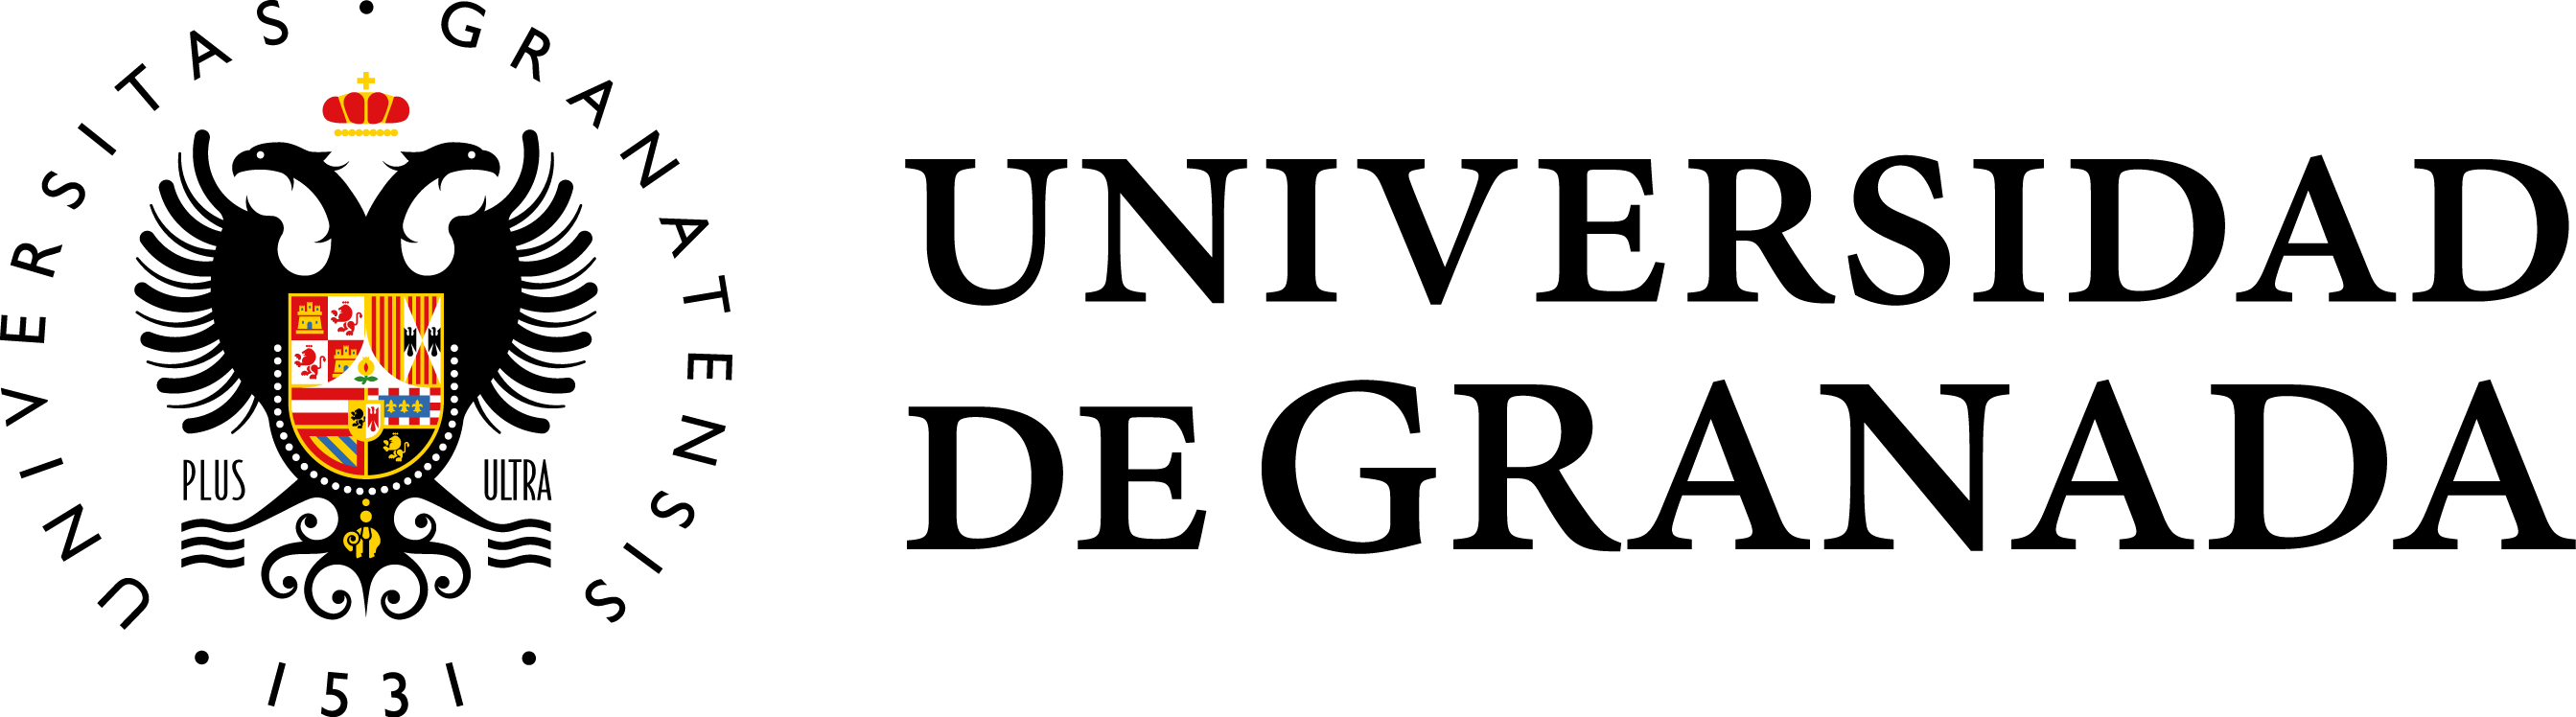
\includegraphics[width=6cm]{ugr} \hspace{2.5cm} 
\includegraphics[width=3cm]{FEETCE}}
\end{figure}
\end{center}
\end{titlepage}

\newpage
\tableofcontents
\thispagestyle{empty} 
\newpage

\section{\textbf{Descripción del problema}}  
Vamos a crear un sistema de información gestionado por un único administrador que será el encargado de realizar las tareas de añadir, editar y eliminar “plantas“ correspondientes a una especie vegetal concreta que podamos encontrar en el Parque de San amaro de Ceuta. En estas plantas se almacenarán, a parte de imágenes, algunos datos  del encuadre taxonómico de la especie: clase, subclase, orden, familia, género, especie y subespecie.  En relación a las características, se tendrán en cuenta cuál es el tipo de planta (árbol, arbusto...), el tamaño que adquieren en la edad adulta,  la forma de las hojas, características del fruto (carnoso, con semillas...), características de las flores (número de pétalos, disposición de estas...), etc.; con respecto a su ciclo reproductivo se almacenarán la floración, maduración y multiplicación. El objetivo del sistema es ofrecer al usuario una base de datos específica en la que se pueda acotar o saber qué especie es la que se está observando a través de las características físicas que presenta o para ver cuáles presentan unas características concretas. El método de búsqueda se realizará a partir de una característica elegida de un desplegable, mostrando otro desplegable con las encontradas en las bases de datos y a partir de estas saber la cantidad de especies disponibles en el parque, pudiendo añadir características cada vez que se elija una con las concordancias disponibles, por eso nuestro sistema debería indexar las especies teniendo en cuentas las características X, para agilizar la búsqueda en tiempo real, así, al llegar al número aproximado de especies, mostrar los enlaces a las plantas con la búsqueda de usuario. Estas plantas se identificarán por el par género-especie.
\newpage

\section{\textbf{Requisitos del sistema}}

En este apartado se describirán los requisitos del sistema, que dividiremos en cuatro grupos (Datos, funcionales, no funcionales y restricciones semánticas) teniendo en cuenta nuestros principales objetivos:

\begin{enumerate}
\item Acceder a información técnica de la planta a través del nombre o los datos de esta.
\item Mantener una base de datos del parque lo más accesible posible, tanto para gente experimentada como no.
\end{enumerate}

\subsection{\textbf{Requisitos de datos}}

Se listan los datos necesarios para el correcto funcionamiento del sistema.
\newline
\begin{enumerate}[label={RD\arabic*.} ,leftmargin=2.8\parindent]
 
 	\item \underline{Datos para crear una planta}:
	\begin{enumerate}[label={RD1.\arabic*.}]
	
	\item 
		\textbf{Taxonomía:} \textit{clasificación científica de la especie.}
	\begin{enumerate}[label=-]
		\item Clase (cadena de hasta 15 caracteres)
		\item Subclase (cadena de hasta 15 caracteres)
		\item Orden (cadena de hasta 15 caracteres)
		\item Familia (cadena de hasta 15 caracteres)
		\item Género (cadena de hasta 15 caracteres)
		\item Especie (cadena de hasta 15 caracteres)
	\end{enumerate}
	\medskip
	
	\item 
		\textbf{Tipo:} \textit{forma de la planta.} (cadena de 18 caracteres)

	\medskip
	\item
		\textbf{Hoja:}
	\begin{enumerate}[label=-]
		\item Forma (cadena de 12 caracteres)
		\item Color (cadena de 24 caracteres)
		\item Persistencia: \textit{perenne o caduca.} (cadena de 8 caracteres)
	\end{enumerate}

	\medskip	
	\item
		\textbf{Fruto:} \textit{tipo de fruto.} (cadena de 20 caracteres)

	\medskip
	\item
		\textbf{Flor:}
	\begin{enumerate} [label=-]
		\item Color (cadena de 24 caracteres)
		\item Forma (cadena de 16 caracteres)
		\item Disposición: \textit{agrupado o solitario.} (cadena de 10 caracteres)
		\item Número de pétalos (número entero de 2 dígitos)
	\end{enumerate}
	
	\medskip
	
	\item
		\textbf{Tamaño:} \textit{tamaño aproximado en la edad adulta.}
	\begin{enumerate}[label=-]
		\item Altura (númerico float, 6 dígitos, 3 decimales, en cm)
	\end{enumerate}
	
	\medskip	
	\item
		\textbf{Imagen:} \textit{imagen de la especie en formato PNG.}

	\medskip 
	\item
		\textbf{Origen:} \textit{lugar de procedencia.} (cadena de 10 caracteres)
		
	\medskip 
	\item
		\textbf{Ciclo reproductivo:}
	\begin{enumerate} [label=-]
		\item Floración (tipo date con mes inicial y final)
		\item Maduración (tipo date con mes inicial y final)
		\item Multiplicación (tipo date con mes inicial y final)
	\end{enumerate}
	\medskip 
	\item
		\textbf{Estado:} \textit{estoy o no en papelera.} (booleano)
	\medskip \medskip
		\end{enumerate}
	
	\item \underline{Datos para editar una planta}:
	\begin{enumerate}[label={RD2.\arabic*.}]
	
	\item 
		\textbf{Tipo:} \textit{forma de la planta.} (cadena de 18 caracteres)

	\medskip
	\item
		\textbf{Hoja:}
	\begin{enumerate}[label=-]
		\item Forma (cadena de 12 caracteres)
		\item Color (cadena de 24 caracteres)
		\item Persistencia: \textit{perenne o caduca.} (cadena de 8 caracteres)
	\end{enumerate}

	\medskip	
	\item
		\textbf{Fruto:} \textit{tipo de fruto.} (cadena de 20 caracteres)

	\medskip
	\item
		\textbf{Flor:}
	\begin{enumerate} [label=-]
		\item Color (cadena de 24 caracteres)
		\item Forma (cadena de 16 caracteres)
		\item Disposición: \textit{agrupado o solitario.} (cadena de 10 caracteres)
		\item Número de pétalos (número entero de 2 dígitos)
	\end{enumerate}

	\medskip
	\item
		\textbf{Tamaño:} \textit{tamaño aproximado en la edad adulta.}
	\begin{enumerate}[label=-]
		\item Altura (númerico float, 6 dígitos, 3 decimales, en cm)
	\end{enumerate}
	
	\medskip	
	\item
		\textbf{Imagen:} \textit{imagen de la especie en formato PNG.}

	\medskip 
	\item
		\textbf{Origen:} \textit{lugar de procedencia.} (cadena de 10 caracteres)
		
	\medskip 
	\item
		\textbf{Ciclo reproductivo:}
	\begin{enumerate} [label=-]
		\item Floración (tipo date con mes inicial y final)
		\item Maduración (tipo date con mes inicial y final)
		\item Multiplicación (tipo date con mes inicial y final)
	\end{enumerate}	
		\medskip 
	\item
		\textbf{Estado:} \textit{estoy o no en papelera.} (booleano)			
	\medskip 
	\medskip
	\end{enumerate}

	\item \underline{Datos para dar de baja una planta}:
	\begin{enumerate}[label={RD3.\arabic*.}]
		\item 
		\textbf{Taxonomía:} \textit{clasificación científica de la especie.}
	\begin{enumerate}[label=-]
		\item Género (cadena de hasta 15 caracteres)
		\item Especie (cadena de hasta 15 caracteres)
	\end{enumerate}
		\medskip 
	\item
		\textbf{Estado:} \textit{estoy o no en papelera.} (booleano)
	\medskip 
	\medskip
	\end{enumerate}
	
	\item \underline{Datos para eliminar una planta}:
	\begin{enumerate}[label={RD4.\arabic*.}]
	
	\item 
		\textbf{Taxonomía:} \textit{clasificación científica de la especie.}
	\begin{enumerate}[label=-]
		\item Género (cadena de hasta 15 caracteres)
		\item Especie (cadena de hasta 15 caracteres)
	\end{enumerate}
	\medskip 
	\item
	\textbf{Estado:} \textit{estoy o no en papelera.} (booleano)
	\medskip 
	\medskip
	\end{enumerate}
	
	\item \underline{Datos para recuperar una planta}:
	\begin{enumerate}[label={RD5.\arabic*.}]
		\item 
		\textbf{Taxonomía:} \textit{clasificación científica de la especie.}
	\begin{enumerate}[label=-]
		\item Género (cadena de hasta 15 caracteres)
		\item Especie (cadena de hasta 15 caracteres)
	\end{enumerate}
		\medskip 
	\item
		\textbf{Estado:} \textit{estoy o no en papelera.} (booleano)	
	\medskip 
	\medskip
	\end{enumerate}
	
	\item \underline{Datos para administrar usuario}:
	\begin{enumerate}[label={RD6.\arabic*.}]
		\medskip
		\item Nombre de usuario (cadena de hasta 8 caracteres)
		\item Correo electrónico (dos cadenas de hasta 15 caracteres y una cadena de tres caracteres con el formato: cadena1@cadena2.cadena3)
		\item Contraseña (cadena de hasta 12 caracteres)
		\item Tipo de usuario (cadena de hasta 15 caracteres)
		\medskip \medskip
		\end{enumerate}

	\item \underline{Datos para iniciar sesión}:
	\begin{enumerate}[label={RD7.\arabic*.}]
		\medskip
		\item Nombre de usuario (cadena de hasta 8 caracteres)
		\item Contraseña (cadena de hasta 12 caracteres)
		\medskip \medskip
		\end{enumerate}

	\item \underline{Datos para recuperar contraseña}:
	\begin{enumerate}[label={RD8.\arabic*.}]
		\medskip
		\item Correo electrónico (dos cadenas de hasta 15 caracteres y una cadena de tres caracteres con el formato: cadena1@cadena2.cadena3)
		\medskip \medskip
		\end{enumerate}
		
 	\item \underline{Datos para buscar una planta}:
	\begin{enumerate}[label={RD9.\arabic*.}]
	
	\item 
		\textbf{Tipo:} \textit{forma de la planta.} (cadena de 18 caracteres)

	\medskip
	\item
		\textbf{Hoja:}
	\begin{enumerate}[label=-]
		\item Forma (cadena de 12 caracteres)
		\item Persistencia: \textit{perenne o caduca.} (cadena de 8 caracteres)
	\end{enumerate}

	\medskip
	\item
		\textbf{Flor:}
	\begin{enumerate} [label=-]
		\item Color (cadena de 24 caracteres)
	\end{enumerate}
		
	\medskip 
	\item
		\textbf{Ciclo reproductivo:}
	\begin{enumerate} [label=-]
		\item Floración (tipo date con mes inicial y final)
	\end{enumerate}
	\medskip
	\item
		\textbf{Estado:} \textit{estoy o no en papelera.} (booleano)	
	\medskip \medskip
		\end{enumerate}
	
 	\item \underline{Datos para consultar una planta}:
	\begin{enumerate}[label={RD10.\arabic*.}]
	
	\item 
		\textbf{Taxonomía:} \textit{clasificación científica de la especie.}
	\begin{enumerate}[label=-]
		\item Clase (cadena de hasta 15 caracteres)
		\item Subclase (cadena de hasta 15 caracteres)
		\item Orden (cadena de hasta 15 caracteres)
		\item Familia (cadena de hasta 15 caracteres)
		\item Género (cadena de hasta 15 caracteres)
		\item Especie (cadena de hasta 15 caracteres)
	\end{enumerate}
	\medskip
	
	\item 
		\textbf{Tipo:} \textit{forma de la planta.} (cadena de 18 caracteres)

	\medskip
	\item
		\textbf{Hoja:}
	\begin{enumerate}[label=-]
		\item Forma (cadena de 12 caracteres)
		\item Color (cadena de 24 caracteres)
		\item Persistencia: \textit{perenne o caduca.} (cadena de 8 caracteres)
	\end{enumerate}

	\medskip	
	\item
		\textbf{Fruto:} \textit{tipo de fruto.} (cadena de 20 caracteres)

	\medskip
	\item
		\textbf{Flor:}
	\begin{enumerate} [label=-]
		\item Color (cadena de 24 caracteres)
		\item Forma (cadena de 16 caracteres)
		\item Disposición: \textit{agrupado o solitario.} (cadena de 10 caracteres)
		\item Número de pétalos (número entero de 2 dígitos)
	\end{enumerate}

	\medskip
	\item
		\textbf{Tamaño:} \textit{tamaño aproximado en la edad adulta.}
	\begin{enumerate}[label=-]
		\item Altura (númerico float, 6 dígitos, 3 decimales, en cm)
	\end{enumerate}
	
	\medskip	
	\item
		\textbf{Imagen:} \textit{imagen de la especie en formato PNG.}

	\medskip 
	\item
		\textbf{Origen:} \textit{lugar de procedencia.} (cadena de 10 caracteres)
		
	\medskip 
	\item
		\textbf{Ciclo reproductivo:}
	\begin{enumerate} [label=-]
		\item Floración (tipo date con mes inicial y final)
		\item Maduración (tipo date con mes inicial y final)
		\item Multiplicación (tipo date con mes inicial y final)
	\end{enumerate}
	\medskip \medskip
		\end{enumerate}
	

\end{enumerate}

\subsection{\textbf{Requisitos funcionales}}

Se definen las características del sistema necesarias para realizar las funciones de usuario, en este caso únicamente tenemos al administrador y los usuarios que acceden a los datos.

\bigskip

\begin{enumerate}[label=RF\arabic*. ,leftmargin=2.8\parindent]
	\item \underline{Crear planta}
	 \newline 
	 \newline
	El sistema debe poder crear una planta nueva en el sistema.
	\begin{enumerate}[label=-]
	
		\item Se requiere de los datos de creación de planta(RD1).
		\item El sistema nos permitirá crear una planta nueva con todos los datos relativos a la planta, pudiendo tener valores por defecto en datos no pertenecientes a los datos taxonónicos.
		\item La planta ha de contener los datos taxonómicos de manera obligatoria en las que género-especie no puede coincidir con una planta ya en la base de datos, dato que será la clave primaria e identificación de cada especie.
		
	\end{enumerate}

	\bigskip
	\item \underline{Editar planta}
	\newline \newline
	Se debe permitir la edición de una planta ya creada.
	\begin{enumerate}[label=-]
	\item Se requiere de los datos para editar la planta(RD2).
		\item Se podrán editar los datos referentes a una planta.
		\item Para que la edición se haga efectiva se han de guardar los cambios realizados.
		\item Una vez la planta ha sido editada no se pueden revertir los cambios realizados.

		
	\end{enumerate}

	\bigskip
	\item \underline{Dar de baja planta}
	\newline \newline
	El sistema permite dar de baja de una planta:
	\begin{enumerate}[label=-]
		\item Se requiere de los datos para dar de baja una planta (RD3).
		\item Se puede dar de baja una planta en cualquier momento.
		\item Se ocultará la planta dada de baja en una \textit{"papelera"} durante 7 días.
		\item La planta puede ser enviada a la papelera desde una opción disponible en esta, únicamente disponible para usuarios del sistema.		
		\item Una vez la planta esté en la papelera durante un período de 7 días se eliminará definitivamente.
		\item No se podrá crear una nueva planta con la misma combinación de datos RD1.1 hasta que la planta no haya sido eliminada completamente del sistema.
	\end{enumerate}

	\bigskip
	\item \underline{Eliminación de planta}
	\newline \newline
	El sistema permite eliminar una planta.
	\begin{enumerate}[label=-]
	\item Se requiere de los datos para eliminar planta(RD4).
		\item Si se desea eliminar una planta dada de baja, se podrá hacer desde la papelera.
	\end{enumerate}

	\bigskip
	\item \underline{Recuperación de planta}
	\newline \newline
	Para la recuperación de plantas:
	\begin{enumerate}[label=-]
	\item Se requiere de los datos de recuperación de planta (RD5).
	\item La planta ha de estar en la \textit{"papelera"}.
	\item No se podrá editar una planta mientras se encuentre en la \textit{"papelera"}.
	\end{enumerate}

	\bigskip
	\item \underline{Administración de usuario}
	\newline \newline
	El sistema contará con un usuario.
	\begin{enumerate}[label=-]
	\item Se requiere de los datos para administrar al usuario (RD6).
		\item Deberá iniciar sesión con usuario y contraseña.
		\item La contraseña será recuperable únicamente por correo electrónico de verificación.
		\item No se pueden crear nuevos usuarios en el sistema.
		
	\end{enumerate}

	\bigskip
	\item \underline{Inicio de sesión}
	\newline \newline
	El inicio de sesión permitirá:
	\begin{enumerate}[label=-]
	\item Se requiere de los datos de inicio de sesión (RD7).
		\item Iniciar sesión con usuario administrador desde cualquier navegador web.
		\item Se deberá utilizar la contraseña única.
		\item Una vez se intenta acceder de manera errónea 5 veces, se bloqueará el acceso durante 5 minutos para la dirección desde la que se acceda.
	\end{enumerate}


	\bigskip
	\item \underline{Cierre de sesión}
	\newline \newline
	El inicio de sesión permitirá:
	\begin{enumerate}[label=-]
		\item Se permitirá el cierre de sesión desde la página.
		\item Se cerrará la sesión automáticamente cuando ocurra una pérdida de conexión.
	\end{enumerate}

	\bigskip
	\item \underline{Recuperación de contraseña}
	\newline \newline
	Para recuperar la contraseña:
	\begin{enumerate}[label=-]
		\item Se requieren los datos para recuperar contraseña (RD8).
		\item Se enviará un correo al usuario para la recuperación.
	\end{enumerate}
	
	\bigskip
	\item \underline{Búsqueda en el sistema}
	\newline \newline
	El sistema debe permitir que cualquier usuario acceda a una búsqueda detallada sobre los datos almacenados.
	\begin{enumerate}[label=-]
		\item Se requieren los datos para buscar en el sistema (RD.9).
		\item La búsqueda se podrá realizar a partir de un único dato.
		\item Cada vez que se añade un dato a la búsqueda, el sistema mostrará el número de coincidencias.
		\item Las plantas que coincidan se mostrarán por el par género-especie y su fotografía.
		\item Los resultados se mostrarán por orden alfabético.
	\end{enumerate}
		
	\bigskip
	\item \underline{Consultar planta}
	\newline \newline
	El sistema permitirá acceder a la información completa de una planta contenida en la base de datos:
	\begin{enumerate}[label=-]
		\item Se requieren los datos de acceso a planta (RD.10).
		\item Para acceder a una planta se ha de haber realizado una búsqueda.
		\item Se accederá a una planta concreta clicando sobre la previsualización de ésta.
		\item Sólo se mostrará una planta completa por pantalla, pudiendo navegar a la siguientes resultantes de la búsqueda a través de flechas dispuestas en los laterales.
	\end{enumerate}
	
\end{enumerate}

\subsection{\textbf{Requisitos no funcionales}}

Se detallan a continuación los requisitos no funcionales del sistema.
\newline

\begin{enumerate}[label=RNF\arabic*. ,leftmargin=3.2\parindent]
	
	\item Rendimiento:
		\begin{enumerate}[label=-]
			\item Se limitará el número de imágenes contenidas en cada planta a 3.
			\item Se crearán índices de búsqueda para agilizar el número de casos antes de mostrar la previsualización en la búsqueda.
		    
		\end{enumerate}
		
	\item Interfaz:
		\begin{enumerate}[label=-]
			\item El usuario final se comunicará con el sistema vía web.
			\item El sistema se comunicará con la base de datos contenedora de la información almacenada.
		\end{enumerate}
	
	\item Escalabilidad:
		\begin{enumerate}[label=-]
			\item El sistema admitirá posteriormente la creación de nuevos usuarios.
		\end{enumerate}
	
\end{enumerate}

\subsection{\textbf{Restricciones semánticas}}

Se exponen las restricciones semánticas sobre el sistema:
\newline

\begin{enumerate}[label=RS\arabic*. ,leftmargin=2.8\parindent]
	
	\item El par género-especie es único para cada planta.
	\item Las plantas pueden ser creadas/editadas/eliminadas por un único administrador.
	\item El tamaño máximo de una imagen será de 250KB.
	\item La contraseña ha de contener un valor numérico y un caracter especial.
	\item El usuario administrador es el único que puede acceder a la \textit{"papelera"}.
	\item Durante la búsqueda no se tienen en cuenta aquellas plantas que se encuentren en la \textit{"papelera"}.
	\item El correo electrónico para la recuperación ha de ser válido.
	
\end{enumerate}
\newpage 

\section{\textbf{Diagramas}}

\subsection{\textbf{\textit{Esquema de caja negra}}}

\begin{figure} [h]
\centering 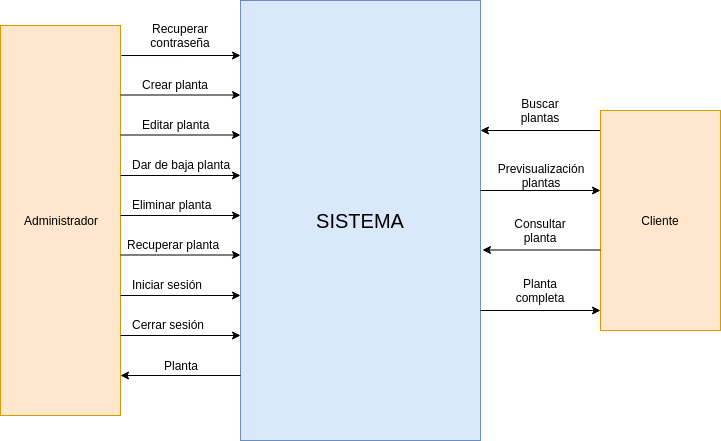
\includegraphics[width=13cm, keepaspectratio]{CajaNegra}
\caption{Esquema de caja negra}
\end{figure}

\subsection{\textbf{\textit{Esquema funcional de armazón}}}

\begin{wrapfigure}[11]{l}{10cm}
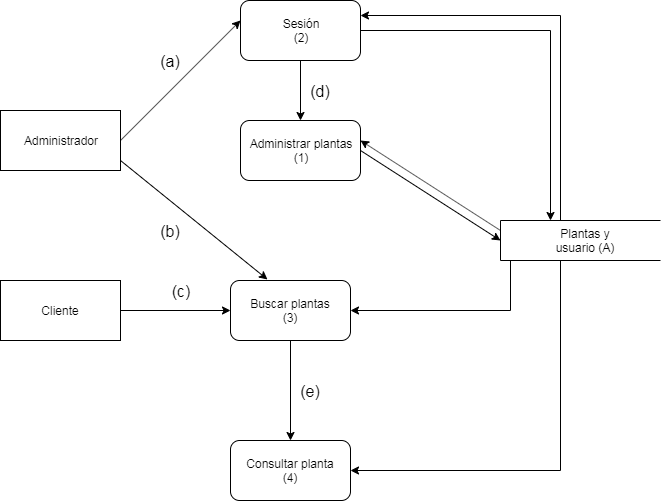
\includegraphics[width=10cm, keepaspectratio]{Armazon}
\caption{Esquema funcional de armazón[DFD(0)]}
\end{wrapfigure}


\textbf{Leyenda:}

	\begin{enumerate} [label=\alph*)]
	\item 
		\medskip
		\begin{itemize}[label=-]
			\item Iniciar sesión
			\item Recuperar contraseña		
		\end{itemize}
	\item 
		\medskip
		\begin{itemize}[label=-]
			\item Buscar plantas		
		\end{itemize}

	\item 
		\medskip
		\begin{itemize}[label=-]
			\item Buscar plantas		
		\end{itemize}
		
	\item 
		\medskip
		\begin{itemize}[label=-]
			\item Crear planta
			\item Editar planta
			\item Dar de baja planta
			\item Eliminar planta
			\item Recuperar	
		\end{itemize}
		
	\item
		\medskip
		\begin{itemize}[label=-]
			\item Consultar planta
		\end{itemize}

	\end{enumerate}
\newpage

\subsection{\textbf{\textit{Refinamientos}}}
\begin{wrapfigure}[11]{l}{10cm}
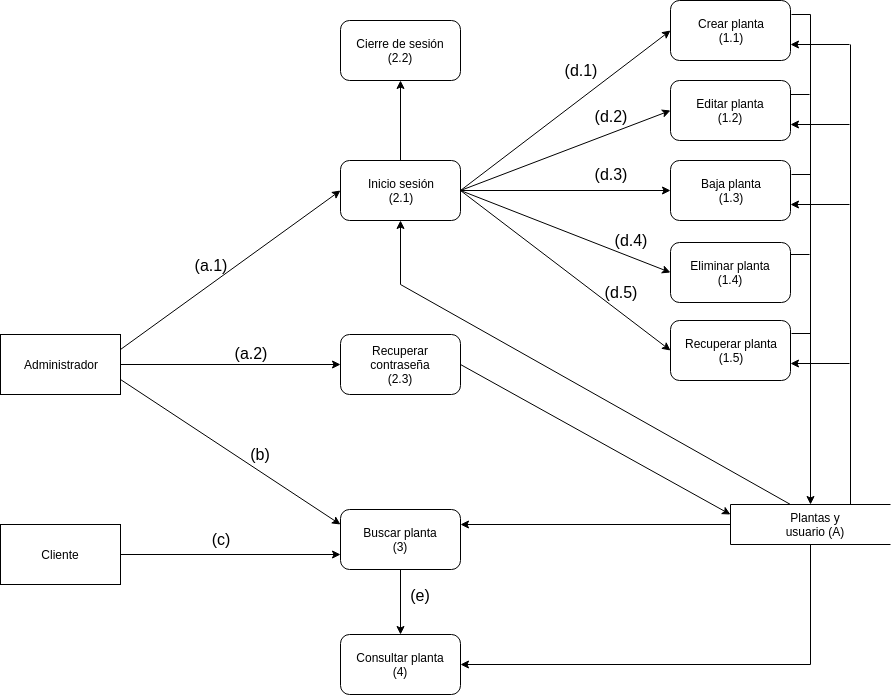
\includegraphics[width=10cm, keepaspectratio]{DFD1}
\caption{Primer refinamiento[DFD(1)]}
\end{wrapfigure}


\textbf{Leyenda:}

	\begin{itemize}[label=]
		\item a.1) Iniciar sesión
		\item a.2) Recuperar contraseña \\
		\item b) Buscar plantas \\
		\item c) Buscar plantas \\
		\item d.1) Crear planta
		\item d.2) Editar planta
		\item d.3) Dar de baja planta
		\item d.4) Eliminar planta
		\item d.5) Recuperar planta\\
		\item e) Consultar planta
	\end{itemize}
	
\vspace{3cm}

\begin{wrapfigure}[11]{l}{10cm}
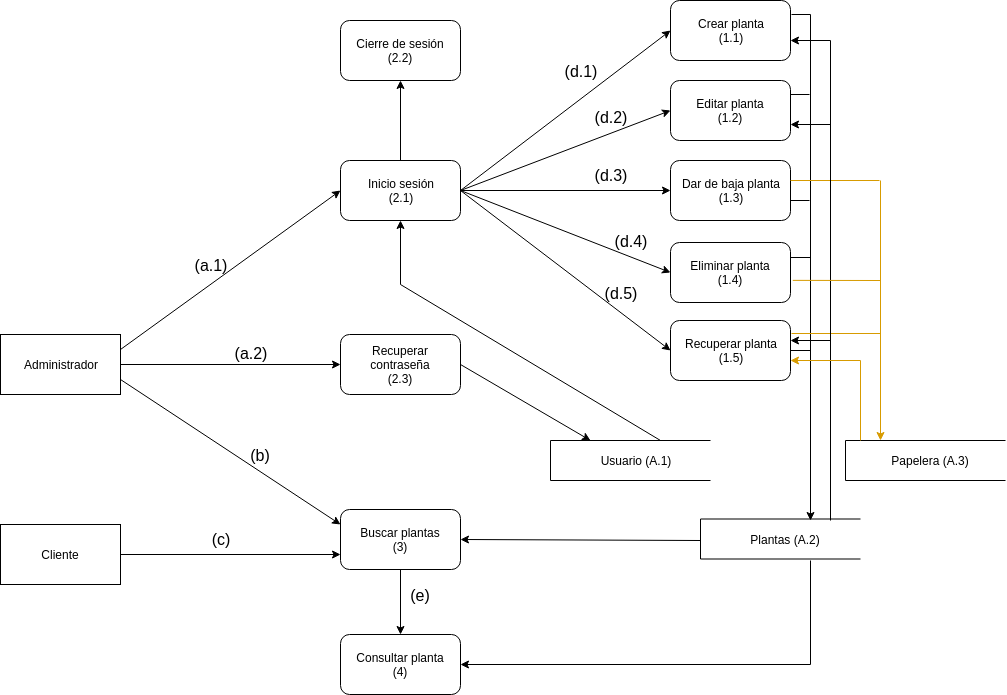
\includegraphics[width=10cm, keepaspectratio]{DFD2}
\caption{Segundo refinamiento [DFD(2)]}
\end{wrapfigure}


\textbf{Leyenda:}

	\begin{itemize}[label=]
		\item a.1) Iniciar sesión
		\item a.2) Recuperar contraseña 
		\item b) Buscar plantas 
		\item c) Buscar plantas 
		\item d.1) Crear planta
		\item d.2) Editar planta
		\item d.3) Dar de baja planta
		\item d.4) Eliminar planta
		\item d.5) Recuperar planta
		\item e) Consultar planta
	\end{itemize}

\newpage
\subsection{\textbf{\textit{Diagrama Entidad-Relación}}}


\begin{figure} [h!]
%fit page keeping ratio: width=\textwidth, height=\textheight, keepaspectratio
\centering 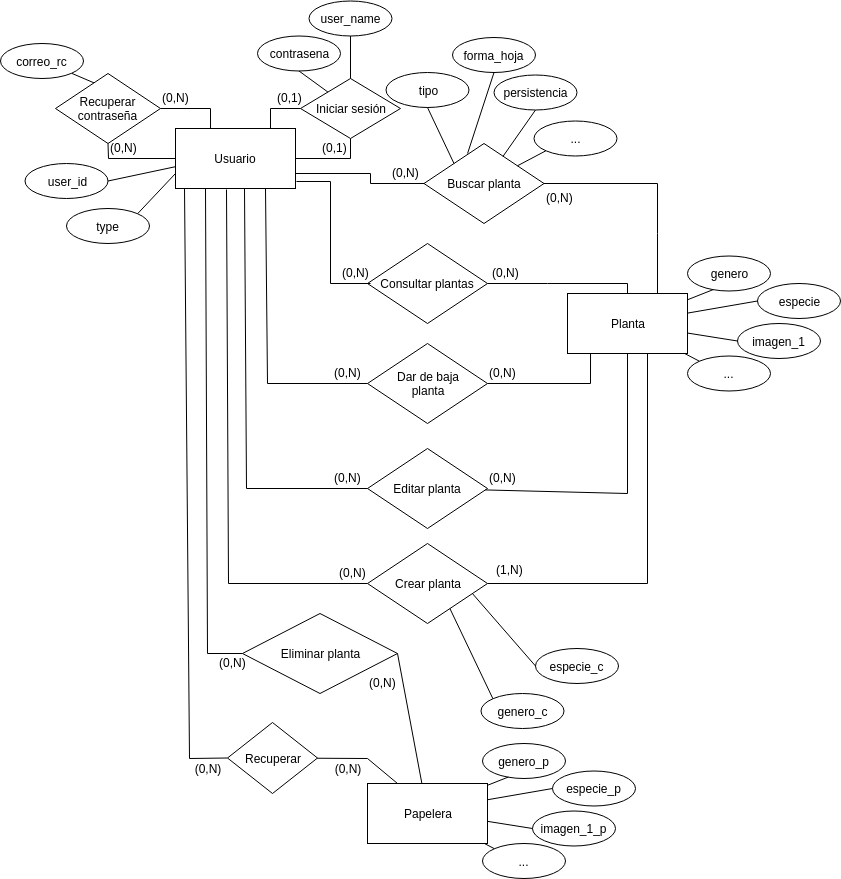
\includegraphics[width=\textwidth, height=\textheight, keepaspectratio]{DER}
\caption{Diagrama Entidad-Relación}
\end{figure}

\end{document}
